% !TEX root = ../thesis-example.tex
%
\chapter{Evaluation}
\label{sec:evaluation}

The evaluation of this project was split into three categories. A system usability evaluation of the web app was conducted to gather data on it's intuitiveness and ease of use, a testing suite was created to evaluate robustness of the web server and it's responses when operating the bot and platform and an empirical study of different strategies and their parameters to provide comparisons on their performances. These categories cover all parts of development of this project and evaluate them appropriately.


\section{Web App Usability}
\label{sec:evaluation:ui}
\noindent The purpose of the system usability evaluation aims to identify if the web app is intuitive for new and experienced users to the cryptocurrency market and evaluates the implementation of the front end (Sec. \ref{sec:implementation:frontend}, pg. \pageref{sec:implementation:frontend}). The candidates level of knowledge on cryptocurrencies and their experience of using cryptocurrency or stock markets was recorded to identify how the web app is used with these different levels of experience, and what issues the candidates faced. The evaluation required the candidate to complete tasks using the web app and to provide feedback and rate the tasks while being observed. The tasks tested how the web app presents,
\begin{enumerate}
\item Coin pair information
\item Controls for the bot
\item Trade signals 
\item Strategy configurations
\item Feedback on operations executed by the bot
\item Selection of different coin pairs
\item Live market depth
\end{enumerate}

% TASK 1 IN EVAL

\noindent To analyse how the web app presents coin pair information, candidates were tasked with gathering information about what coin pair was currently selected, the last traded price, the highest and lowest 24 hour price and the total volume traded in 24 hours. My initial hypothesis for completing this task was to be relatively straightforward as all this information is contained at the top of the web app. While this was partially true, this result mainly came from users who state they had atleast some experience using a cryptocurrency exchange. One candidate stated, "All the data was available on the top of the screen where your eyes naturally look for the information if you have used any form of stock trading." Another states, "Naturally, I looked at the top of the screen as that is where a price ticker tends to be on a cryptocurrency exchange."

However, some candidates who have only heard of cryptocurrency exchanges but have never used one struggled with this. One candidate tried to find this data within the candlestick chart and coin pair listings, which does display relevant data, but not clearly or easily. This candidate did complete the task after noticing the top bar but stated "I am new to trading platforms, the GUI [\textit{appears to be}] busy and can be overwhelming. However, after a few minutes, you begin to get a feel for it and know what each section represents." 

% TODO may need updated with more candidates, maybe charts as well?
Candidates could rate this task between 1 (Very difficult) and 5 (Very easy), where most rated it at a 5. This shows this design is intuitive and familiar with most candidates and suggests that understanding how to derive specific data from the panels is straightforward. Although, for inexperienced users, the initial learning curve looks to be the biggest issue with the lowest rating rated at a 2. This seems to persist as a repeating issue throughout this evaluation.

From this first task, a clear distinction in knowledge attributes to the different approaches of completing it. Inexperienced users felt lost and overwhelmed within the UI and struggled to derive data displayed at the top of the page initially, whereas experienced users spotted this panel straightaway. A future solution to solve this issue may be to introduce a \textit{one-time pop up}. This pop up would occur on a users first visit to the page and present a quick description over each section of the UI. This would give the user a basic knowledge of what information the user is presented with and how to understand it as to allow them to be familiar with the web app as quick as possible.

% TASK 2 AND 4 IN EVAL
\noindent Candidates were tasked to start the bot and then stop the bot in a later task. These tasks were issued separately and non-sequentially as they both require a similar approach to completing them. This can bring a measure to how candidates approach the web app as they become more familiar with it. All candidates found the button easy to identify when trying to locate it to start and stop the bot.

Candidates were also requested to provide feedback about how they could confirm the bot had successfully completed this operation and if they felt informed about what the bot's current status was. Most candidates found that the snackbar (pop-up) notification was helpful in confirming the bot had completed the operation and that it was not intrusive on the web app. Some candidates noted on the button being a toggle for the operations and that it was "natural to click it again to turn it off". This provides clear testimonials that basic bot operations are concise and natural for a user to understand.

After completing each task, candidates were asked to rate how clearly they were informed of the bots status on a scale between 1 (Very unclear) and 5 (Very clear). Most rated 5, stating that they were informed very clearly. However, one candidate, who describes themselves as spending a lot of time using cryptocurrency exchanges, rated 3 on the first task. On the second task that required the candidate to stop the bot, they increased their rating to a 4. This suggests that after spending time using the web app to complete similar task, a user becomes more familiar with how it operates and feels more informed about what to expect from the web app. This further confirms that their is a learning curve to using the web app and that users can become more familiar with it as they spend time using it.

This outcome is interesting however as this candidate has experience of cryptocurrency exchanges where their likeness pertains to this web app, yet they were one of the only candidates that did not feel they were clearly informed. This candidate left feedback after completing the first task stating, "The indicators don't give a lot of context as to what is happening, it requires some working out to realise that they obviously say \textit{up} and \textit{down}." While the indicators the bot generated on the candlestick chart were not a part of this task, only two candidates - both of whom are experienced with cryptocurrency exchanges - noticed the effect the bot had on the candlestick chart after starting it. The other candidate noted they felt very informed of the bot's current status even after noticing the signal indicators on the candlestick chart, so this may be the result of whether the first candidate felt informed about what the bot had displayed on the candlestick chart rather than what the bot's current status actually was. This will be discussed further in the trade signals discussion below.

A final point to make on these tasks is the little mention of the operational messages panel. No candidate noted on it, favouring to look at the snackbar notification solely. This panel is important for keeping a log of current and past events as to allow a user to stay fully informed of all recent actions. This presents the issue that when important and descriptive notifications are displayed on this panel, they may be overlooked by the snackbar, which by design only highlights a high level overview message. A few solutions to making the push message panel more prominent could be to prevent the snackbar overlapping it, to add a transition animation for when a new message is received and to make it more attractive through colours. 

\noindent 


% Evaluation of the front end implementation will be compared towards the functional requirements \textbf{FR-1, FR-2, FR-3, FR-4, FR-5, FR-6, FR7, and FR-8} in table \ref{table:requirements:func} (Pg. \pageref{table:requirements:func}). As these requirements have been catered towards the aims and objectives, this will validate the completion of the project.


\section{Web Server Testing}
\label{sec:evaluation:web_server}

\noindent An evaluation of the web server's robustness and ability to respond to events is tested through unit tests on all of the available endpoints and can be used to draw conclusions on the implementation of the information and communications process (Sec. \ref{sec:implementation:info_comm}, pg. \pageref{sec:implementation:info_comm}). Specifically, this section looks to evaluate the process performed by the part of the web server that handles the forwarding of data received from Binance to the user. This includes when the 429 status code is received or an API restriction is in affect. Testing of the web server's communication between a user and a bot is also performed by testing if input is validated, if the responses are appropriate for the outcome of the operation and if API restrictions are handled appropriately. There are 10 unit tests in total that cover the exceptions stated above that the web server may encounter during operation, however this is a non-exhaustive list.


\subsection{Exchange Data Endpoints}
\label{sec:evaluation:web_server:exch_data}
% Unit tests on data end points

% TODO update the 'listed requirement'
\noindent Retrieving exchange data from Binance in a controlled and non-abusive manner is one of the listed requirements of this project. This means that the 429 status code that can be received from Binance is required to be handled appropriately through the implemented self-ban functionality. Therefore, the unit tests listed in table \ref{sec:evaluation:web_testing:exch_data:all_tests} have been created to confirm this functionality works robustly. The endpoints listed in table \ref{sec:evaluation:web_testing:data_apis} and \ref{sec:evaluation:web_testing:data_ws} are some of the web server's Binance data endpoints that are tested by the unit tests in table \ref{sec:evaluation:web_testing:exch_data:all_tests} because they perform API requests to Binance. 

\begin{table}[ht]
\centering
  \begin{tabularx}{\linewidth}{|c|c|L|c|} 
    \hline
    \textbf{ID} & \textbf{Endpoint Type} & \textbf{Description of Test} & \textbf{Outcome} \\ 
    \hline\hline
    1  & API & Spam the \textbf{allCurrencyPairs} endpoint until a non-200 request is returned. & Pass    \\ 
    \hline
    2  & API &   Spam the \textbf{orderbook} endpoint until a non-200 request is returned.  & Pass    \\ 
    \hline
    3  & WebSocket & Trigger the \textbf{connect} event of the \textbf{candlestick} endpoint when a self-ban has occurred & Pass    \\ 
    \hline
    4  & WebSocket &  Trigger the \textbf{get\_klines} event of the \textbf{candlestick} endpoint to stream data when a self-ban has occurred. & Pass    \\
    \hline
  \end{tabularx}
\caption{Binance Data Endpoint's Unit Tests and Results}
\label{sec:evaluation:web_testing:exch_data:all_tests}
\end{table}

\noindent Unit tests 1 and 2 in table \ref{sec:evaluation:web_testing:exch_data:all_tests} test the endpoints 1 and 2 in table \ref{sec:evaluation:web_testing:data_apis} respectively. Each endpoint has a fetch request repeatedly sent until a non-200 status code response is returned; due to a 200 status code representing an OK (normal) response. The web server is then expected to return a 429 status code response that is received from Binance to inform the user that the web server is currently restricting API requests. To confirm the self-ban is fully in place, another fetch request is sent immediately after to retrieve data from the endpoint, where another 429 status code is expected to be returned again.

When the 429 status code is ultimately returned to the user who originated the request, it confirms that the web server has appropriately handled the setting or abiding of an API restriction. This is because that, by design of how the web server handles requests, a 429 status code can only be returned from the web server when it has restricted itself from API requests. However, in production this could lead to abuse of the API and ultimately restrict the web server from requesting data entirely. Therefore, a solution for this project could be to either implement an endpoint weighting system similar to the system Binance has, or store local caches of data that are frequently requested to prevent requiring extra calls to their API for the same data another user has requested. 

% TODO maybe compare either solution, does either aid to the objectives or the current project?
While the first party endpoint weighting solution would prevent abuse and lower the chance of requiring self-bans, it would fail to support a large number of concurrent users who would still require requests to gather the data. Implementing this alongside the caching solution would prevent abuse to the web servers endpoint and reduce API calls to Binance as well. This would also further the projects objective of creating a robust web app that can handle varied exception cases.

\begin{table}[ht]
\centering
  \begin{tabularx}{\linewidth}{|c|c|L|} 
 \hline
\textbf{ID} & \textbf{Endpoint URL} & \textbf{Description} \\ 
\hline\hline
1  &   \textbf{allCurrencyPairs} & Returns overview data of all coin pairs.    \\ 
\hline
2  &  \textbf{orderbook@<coin-pair>} & Takes parameter \textit{<coin-pair>} (e.g. `BTCUSDT') and returns current orders in the order book for that coin pair.    \\ 
\hline
\end{tabularx}
\caption{API Endpoints for Binance Data
\textbf{NOTE :} All endpoints are prefixed with \textit{\textbf{"/api/v1/"}}}
\label{sec:evaluation:web_testing:data_apis}
    \end{table}

\noindent Unit tests 3 and 4 in table \ref{sec:evaluation:web_testing:exch_data:all_tests} test the sole WebSocket endpoint that requests data from Binance's API during its events. This occurs during the \textbf{connect} and \textbf{get\_klines} events of the \textbf{kline} namespace (described in table \ref{sec:evaluation:web_testing:data_ws}), therefore a unit test was created for each event. Both events ultimately return a JSON response with the key \textbf{status\_code} that has the value \textbf{429} when it encounters the self-ban restriction. This provides context as to why the operation was unable to complete and provides the interface that uses the endpoint with a way to handle the response appropriately.

The exception responses from the data endpoints currently don't provide any other data other than the keys \textbf{status\_code} and \textbf{msg}. In future works, the web server could return a response to generate a log message, as discussed in section \ref{sec:implementation:frontend:controls_notifications} (Pg. \pageref{sec:implementation:frontend:controls_notifications}), to alert the user that the service is temporarily unavailable. This could also be tied in with the implementation of the web servers own endpoint weighting system to provide updates to the user about any issues the web server is facing or what restrictions are being applied to them. Working examples of this are already implemented in the bot's controller endpoints discussed in section \ref{sec:evaluation:web_server:bot_controls} below.

\begin{table}[ht]
\centering
  \begin{tabularx}{\linewidth}{|c|c|L|} 
    \hline
    \textbf{ID} & \textbf{ \textit{namespace}@\textit{event}} & \textbf{Description} \\ 
    \hline\hline
    1  &   \textbf{kline@connect} & Initial connection to candlestick data's namespace. Performs an API fetch to Binance to confirm its online and serving data. \\ 
    \hline
    2  & \textbf{kline@get\_klines} & Takes coin pair (e.g. BTCUSDT) as data on triggering this event. Performs initial API fetch to Binance for historic data, then creates a WebSocket connection to Binance's WebSocket endpoint and streams the historic and new data back to client who triggered the event. \\ 
    \hline
  \end{tabularx}
\caption{WebSocket Endpoints for Binance Data: 
\textit{(a)} \textbf{\textit{namespace}} is the url for the WebSocket \textbf{NOTE :} All namespaces are prefixed with \textit{\textbf{"/ws/binance/"}}
\textit{(b)} \textbf{\textit{event}} is the event that can be triggered on the namespace to perform a certain action }
\label{sec:evaluation:web_testing:data_ws}
\end{table}

\subsection{Bot Control Endpoints}
\label{sec:evaluation:web_server:bot_controls}
% Unit tests on bot end points

\noindent To ensure robustness of the endpoints that control operations that a user can perform on a bot, a range of test cases are used to test the responses returned by the web server. The test cases listed in table \ref{sec:evaluation:web_testing:bot_controls:all_tests} cover how a bot handles a 429 code that is received from the web server, input validation on data arguments sent to the web server and the normal operations of controlling a bot.

\begin{table}[ht]
\centering
  \begin{tabularx}{\linewidth}{|c|c|L|c|} 
    \hline
    \textbf{ID} & \textbf{Endpoint Type} & \textbf{Description of Test} & \textbf{Outcome} \\ 
    \hline\hline
    1  & API & Start and stop the bot under normal conditions. & Pass    \\ 
    \hline
    2  & API &  Start the bot with missing arguments. & Pass    \\ 
    \hline
    3  & WebSocket & Start the bot under normal conditions. & Pass    \\ 
    \hline
    4  & WebSocket & Start the bot with missing arguments. & Pass    \\ 
    \hline
    5  & WebSocket & Start the bot with no data. & Pass    \\ 
    \hline
    6  & WebSocket & Start the bot with data an API restriction in affect. & Pass    \\ 
    \hline
  \end{tabularx}
\caption{Bot Endpoint Unit Tests and Results}
\label{sec:evaluation:web_testing:bot_controls:all_tests}
\end{table}

Endpoint 1 in table \ref{sec:evaluation:web_testing:bot_apis} and \ref{sec:evaluation:web_testing:bot_ws} interface with the bot in the same way but provide access through two different protocols. While endpoint 1 in table \ref{sec:evaluation:web_testing:bot_apis} is unnecessary for the scope of this project, it is still being discussed and tested here for possible future work. Having this endpoint tested and available allows access from other interfaces that may not support WebSockets but can still communicate through HTTP endpoints. 
\begin{table}[ht]
\centering
  \begin{tabularx}{\linewidth}{|c|c|L|} 
    \hline
    \textbf{ID} & \textbf{Endpoint URL} & \textbf{Description} \\ 
    \hline\hline
    1  &   \textbf{bot/start} & Returns overview data of all coin pairs.    \\ 
    \hline
    2  &  \textbf{bot/stop@<hash-id>} & Takes parameter \textit{<hash-id>} (e.g. "fa25f6...") and returns response appropriate to the outcome of the operation.    \\ 
    \hline
  \end{tabularx}
\caption{API Endpoints for Bot Control 
\textbf{NOTE :} All endpoints are prefixed with \textit{\textbf{"/api/v3/"}}}
\label{sec:evaluation:web_testing:bot_apis}
\end{table}

Unit tests 1 and 3 in table \ref{sec:evaluation:web_testing:bot_controls:all_tests} check whether the bot can start under normal conditions. These tests are useful to confirm if any changes to the project may have affected the start or stop controls of a bot. The initialisation can be executed with the WebSocket or API endpoint, but the WebSocket endpoint is the main endpoint used due to the streaming of signal data to the front end UI. The WebSocket test checks that two JSON responses are received from the server containing the two different message types, as discussed in section \ref{sec:implementation:frontend:controls_notifications} (Pg. \pageref{sec:implementation:frontend:controls_notifications}). 

% TODO add code snippets of expected JSON responses of logs
The log message type holds the import data about the outcome of this endpoint, containing the key \textbf{success} that has the value \textbf{true} when the bot has started, or \textbf{false} if it failed to do so. The bot's unique hash ID is also a part of this response and is confirmed that it has been received while ensuring it is a length of 32 characters. The snackbar message type provides styling information for the pop up message of the frontend by having the key \textbf{variant} with the value \textbf{success}. This provides details about what kind of message the UI should display, in this case a green \textit{success} message.

Unit test 1 in table \ref{sec:evaluation:web_testing:bot_controls:all_tests} is checked for the same data, however only one response is possible and does not have a specific message type. This endpoint is a more direct method to interacting with the bot and its response is not decorated for the front end UI. This endpoint is useful for interfaces that may want to interact with the web server through there own third party service, similar to how this web server interacts with Binance's server. 

Unit test 2 and 4 in table \ref{sec:evaluation:web_testing:bot_controls:all_tests} attempt to the start the bot with missing arguments. The initial testing using test case 4 resulted in the case failing as there was no proper input validation implemented for the WebSocket endpoint, but the API endpoint had built-in functionality to validate its own input. Thus, to ensure consistency with the API when unexpected input was sent to the web server, the WebSocket was re-factored to handle inputs in a similar fashion to the API. This required creating a function to parse the data retrieved and perform basic checks that all the arguments were present. 

Unit test 4 was originally failing as success messages were received, which would be the same results that would pass unit test 3. This obviously would be an incorrect result for when data is missing and therefore it is correct that the test failed. To create a passing result, unit test 4 should require two message types, with the log type returning the key \textbf{success} containing the value \textbf{false} stating the bot failed to start and with the key \textbf{botHash} also containing the value \textbf{none} because the bot did not successfully start. The key \textbf{missing\_args} is also returned with a list of what arguments are missing. This provides an easy way to define what parameters are missing from this endpoint which creates a more maintainable and informative response. 

Unit test 5 in table \ref{sec:evaluation:web_testing:bot_controls:all_tests} attempted to start the bot with no data at all. The re-factor discussed above did not handle data that was fully missing and therefore required the endpoint to be re-factored further. This unit test now expects the key \textbf{success} to be returned with the value \textbf{false} and the key \textbf{msg} to return an appropriate explanation about why the bot failed, which in this case returns, \textbf{"Bot failed to start, no data was received."} This endpoint conforms to an acceptable level of robustness and provides informative data to a bad request. 

Unit test 6 tests a bot that is started through a WebSocket and receives a 429 status code from the web server's candlestick endpoint (2 in table \ref{sec:evaluation:web_testing:data_ws}) for Binance data. The bot would still start as usual and return the same messages that were discussed for unit test 3, but after the bot creates a connection to the candlestick endpoint, three responses are expected to be returned. The first two are the log and snackbar messages to inform the user on the front end that the bot couldn't gather data due to an API restriction and should retry later. The third response is an event call for the front end that triggers the \textbf{stop\_bot} event. This is used to update the UI to inform the user the bot is no longer running. This is important as it allows any interface using the service to handle the event of the server force stopping the bot.

\begin{table}[ht]
\centering
  \begin{tabularx}{\linewidth}{|c|c|L|} 
    \hline
    \textbf{ID} & \textbf{ \textit{namespace}@\textit{event}} & \textbf{Description} \\ 
    \hline\hline
    1  &   \textbf{communicator@bot\_start} & Initial connection to candlestick data's namespace. Performs an API fetch to Binance to confirm its online and serving data. \\ 
    \hline
  \end{tabularx}
\caption{WebSocket Endpoints for Bot Control: 
\textit{(a)} \textbf{\textit{namespace}} is the url for the WebSocket \textbf{NOTE :} All namespaces are prefixed with \textit{\textbf{"/ws/v3/bot/"}}
\textit{(b)} \textbf{\textit{event}} is the event that can be triggered on the namespace to perform a certain action }
\label{sec:evaluation:web_testing:bot_ws}
\end{table}

% \noindent Evaluation of our server infrastructure implementation can be confirmed by our completion of requirements \textbf{NFR-1, NFR-2, NFR-6, and FR-9} in tables \ref{table:requirements:non_func} and \ref{table:requirements:func} (Pg. \pageref{table:requirements:non_func} and \pageref{table:requirements:func}). The analysis undertaken is equivalent to section \ref{sec:evaluation:tradeprocess}.



\section{Strategies Comparison}
\label{sec:evaluation:tradeprocess}

\noindent The range of different strategies will be empirically evaluated and compared against one another by analysing their performance such as the amount of signals generated and the final net value. These strategies will be evaluated on the BTC / USDT coin pair. A mock starting balance of 10,000 USDT (1 USDT = 1\$, hereafter USDT will be represented as \$) will be used for each strategy and a commission rate of 0.1\% will occur on each signal to simulate real transactions that are subject to trading fees on cryptocurrency exchanges. A trade will buy or sell exactly 1 BTC at the closing price of an interval to make the comparisons straightforward. This means that if a buy signal is generated at \$4,800 and a sell signal at \$5,000, the total gross amount would be \$200. This would make the initial portfolio value of \$10,000 become the gross amount \$10,200. Then commission will be subtracted from the \$200 trade it to bring a total net amount.

The strategy's generated signal data has been collected from the \textbf{13-03-19} to the \textbf{10-04-19}, which corresponds to one thousand 30 minute intervals. During this period, the BTC / USDT pair had a significant upward movement in price around three quarters of the way through this period with a mostly sideways moving market throughout the other intervals.

\begin{table}[ht]
\centering
  \begin{tabularx}{\linewidth}{|c|L|c|c|c|} 
    \hline
    \textbf{ID} & \textbf{Strategy Name} & \textbf{Signals Generated} & \textbf{Net Portfolio} & \textbf{Net Profit$/$Loss} \\
    \hline\hline
    \textbf{1} & RSI & 2 & 10,062.00 & 62.00 \\
    \hline
    \textbf{2} & MACD & 105 & 10,239.98 & 239.98 \\
    \hline
    \textbf{3} & SMA Crossover & 51 & 10,614.42 & 614.42 \\
    \hline
    \textbf{4} & MA Crossover \& RSI & 0 & 10,000.00 & 0.00 \\
    \hline
    \textbf{5} & MA Crossover \& MACD & 47 & 10,550.62 & 550.62 \\
    \hline
    \textbf{6} & Bollinger Bands & 25 & 10,925.39 & 925.39 \\
    \hline
    \textbf{7} & Double Bollinger Bands & 1 & 11,501.65 & 1,501.65 \\
    \hline
  \end{tabularx}
\caption{The total number of signals generated and the net portfolio that is resultant of the default parameters for each strategy. The \textbf{Net} column headers are in USDT.}
\label{sec:evaluation:strats:performance}
\end{table}

\noindent Strategy 1  in table \ref{sec:evaluation:strats:performance} shows the performance of the RSI strategy - with the upper threshold at 70 and the lower threshold at 30 - to be quite conserved, generating 2 signals over the month period. The signals also created one of the minimal totals of profit compared to the other strategies at a total of \$62.00. 
The RSI strategy's long signal was generated at the price \$3910.00 and the sell signal at \$3972.00, but looking at the candlestick chart of these signals shows a concerning historic price movement. Before the short signal, the market dipped drastically to only spike and recover. 

As the RSI indicator defines overbought or oversold conditions, it fails to react to the market and therefore could easily have resulted in a significant loss of the portfolio. Furthermore, by looking at the candlestick charts in figure \ref{fig:eval:strats:rsi_signals}, they suggest that a market reversal is not 100\% certain due to the chart price progression following the last short signal. The market actually continues to trend upwards for the rest of the month. The strategy may have benefited from smaller thresholds in this specific instance as the whipsaws between these two signals nearly cross the thresholds but fall short.

\begin{figure}[ht]
  \centering
  \subfloat[Upper threshold 70 and lower threshold 30]{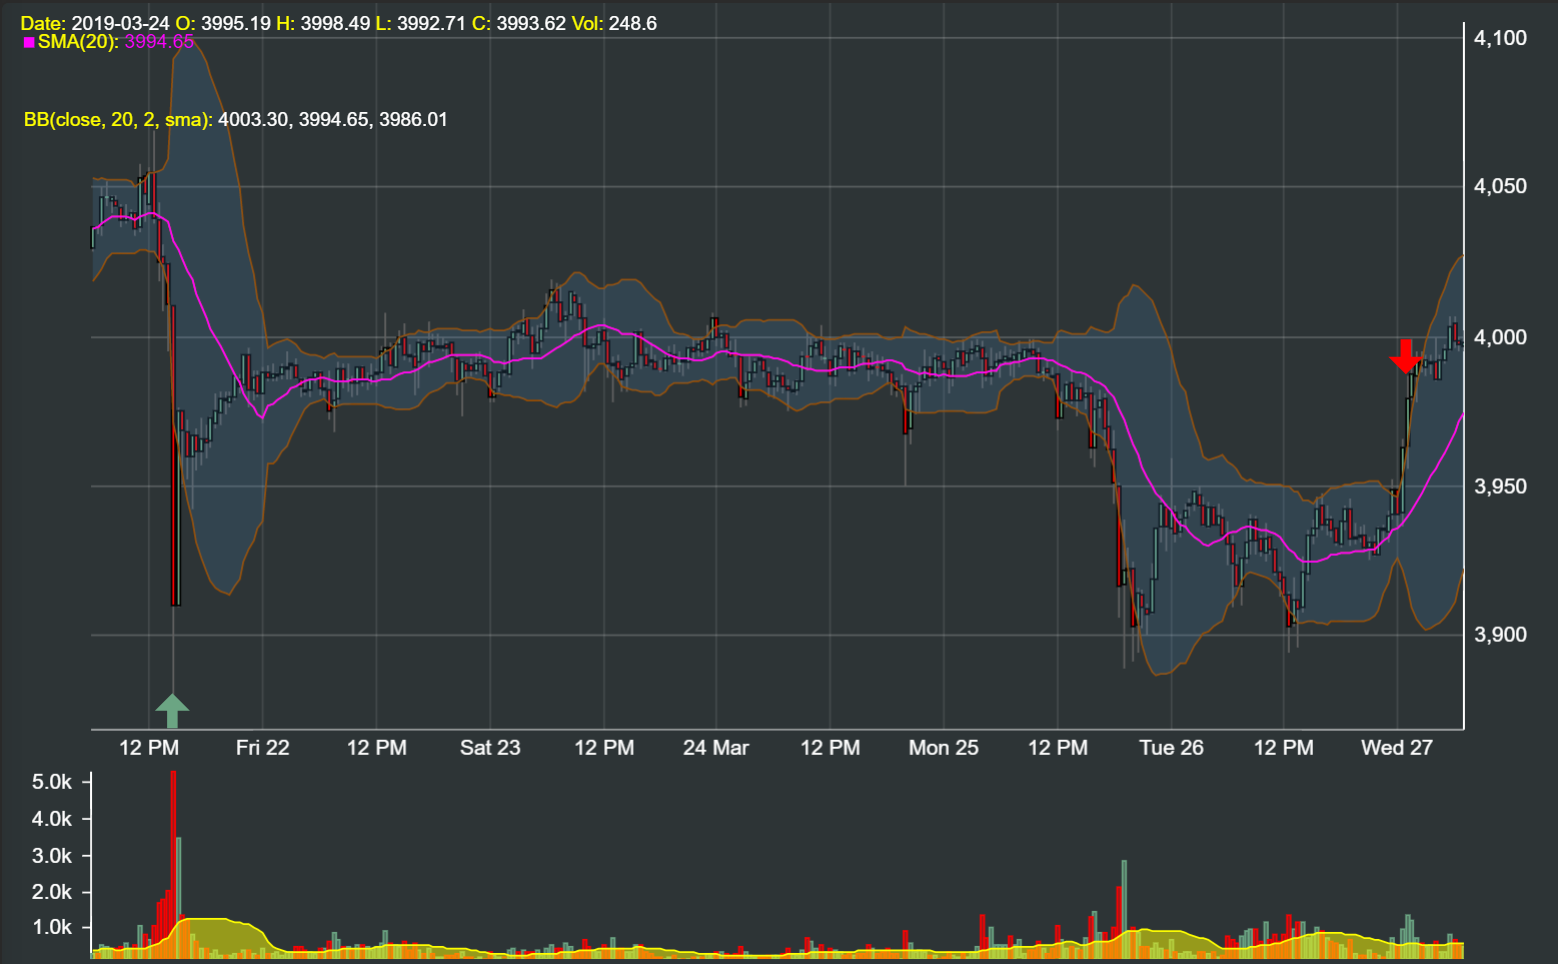
\includegraphics[width=0.49\textwidth]{content/graphics/rsi_default_sg1_sg2.PNG}\label{fig:f1}}
  \hfill
  \subfloat[Upper threshold 60 and lower threshold 40]{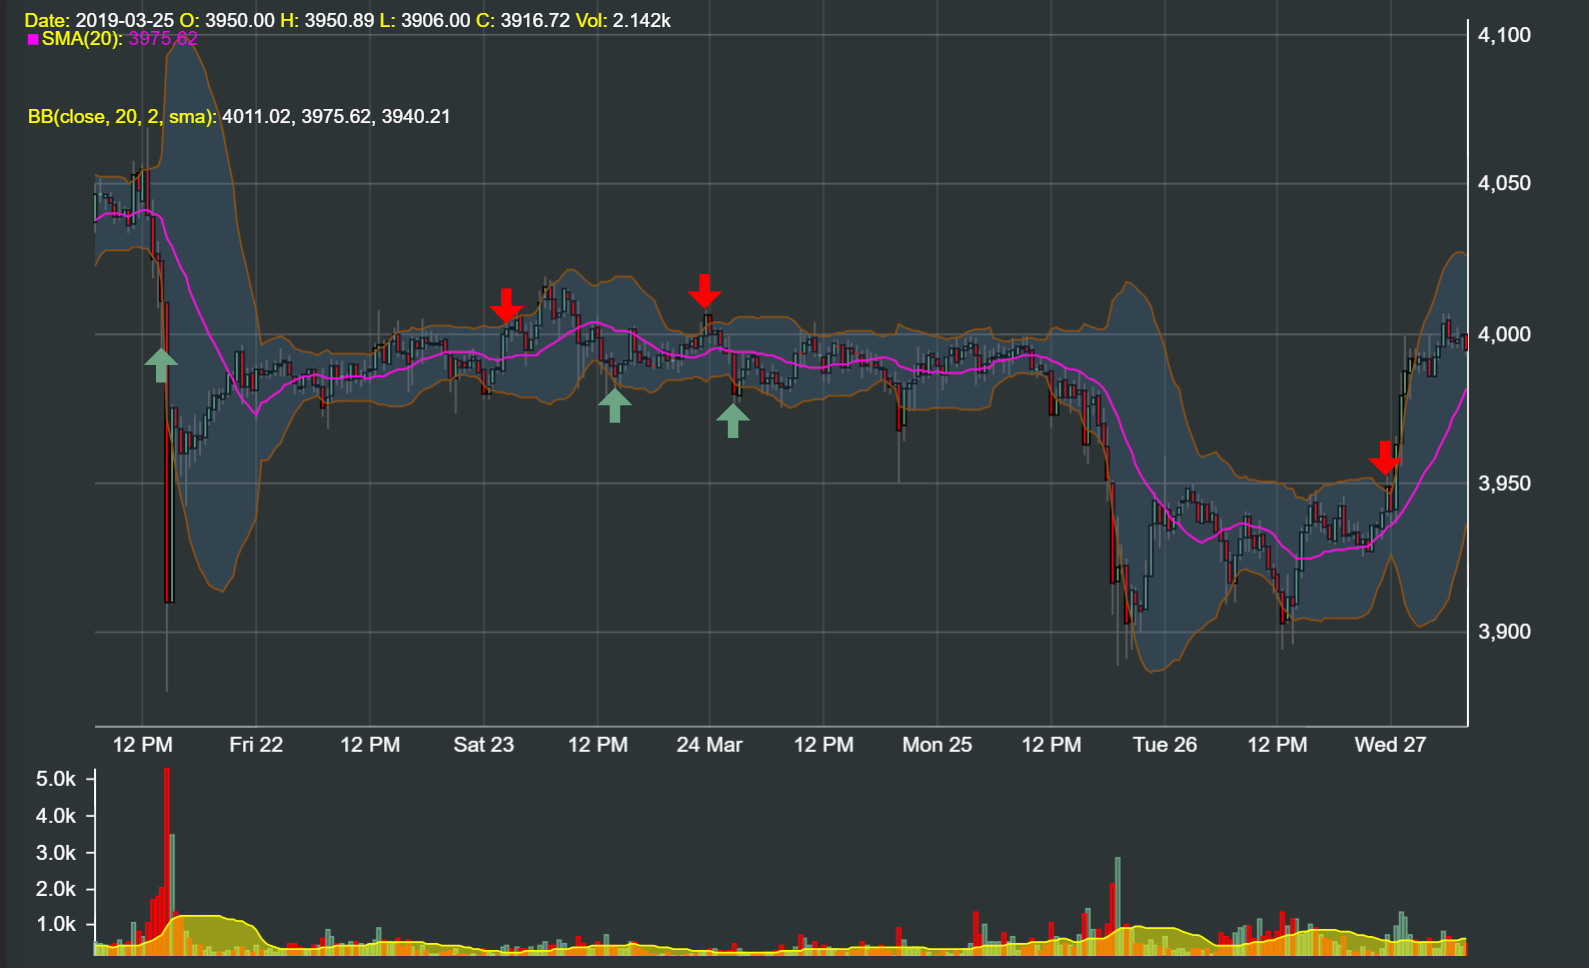
\includegraphics[width=0.49\textwidth]{content/graphics/rsi_60_40_same_period.PNG}\label{fig:f2}}
  \caption{RSI strategy trade signals with different thresholds}
  \label{fig:eval:strats:rsi_signals}
\end{figure}

Specifying the upper threshold at 60 and the lower threshold at 40 actually returns a more profitable strategy. 26 signals are generated rather than 2, with a net portfolio value of \$10,498.73. This is a significant improvement over the default 70 and 30 values. However, comparing the figure \ref{fig:f2} with fig \ref{fig:f1} which span the same period, it is clear that the strategy doesn't find the lowest price of significant drops. The first long signal in figure \ref{fig:f2} is generated before it reaches the lowest price. Although, it does manage to generate the signals within the whipsaws, the lower thresholds still fail to react to the sudden drop off before the last shown signal.

It could be argued that the thresholds at 60 and 40 produce less risk as they generate signals between smaller price ranges. This means that the larger price difference displayed at the 70 and 30 threshold chart would be less likely to occur, reducing the amount of assets being traded at once. Lots of smaller trades also add up as evident by the greater profit gain from the parameters of this strategy. This strategy with the 60 and 40 parameters is still far from perfect however, as the indicators prematurely enter or exit a position before the best price is found.

Strategy 2 in table \ref{sec:evaluation:strats:performance} shows the performance of the MACD indicator to be quite aggressive, generating 105 signals throughout the month period. While displaying an extensively aggressive number of signals over the month, it did generate more profit than the RSI strategy at \$239.98, resulting in \$177.98 more profit. 
 


% \noindent Evaluation of the trade process implementation can be confirmed by our completion of requirements \textbf{NFR-3, NFR-4, and FR-10} in tables \ref{table:requirements:non_func} and \ref{table:requirements:func} (Pg. \pageref{table:requirements:non_func} and \pageref{table:requirements:func}). The analysis undertaken for this evaluation will be a review of the features implemented, provided by code snippets and related outputs. Such evaluations will analyse the use of SMA vs. EMA and applying different RSI thresholds as discussed in section \ref{sec:related:tradingStrategies} (Pg. 11, 12).


\section{Evaluation Review}
\label{sec:evaluation:review}

\noindent The three listed components cover the range of this projects scope. The main focus will be on the Trade Process, swapping in different trade indicators and evaluating their performances. More challenging scopes for evaluation will be the implementation of joing the web app together as whole.